
\chapter{软件测试与分析}

软件测试是验证系统质量、暴露潜在缺陷的关键环节。本章围绕功能测试、兼容性测试和性能测试三大目标对SimpleDesktop系统进行系统化评估，并对测试结果进行客观分析，为系统的最终交付提供质量依据。

\section{功能测试}
\subsection{测试方法与原则}
功能测试采用黑盒测试方法，针对系统对外提供的每一项功能编写测试用例，通过比对实际执行结果与预期结果是否一致来判定功能正确与否。测试遵循覆盖优先、异常优先、边界优先三项基本原则：覆盖优先要求每项功能至少包含一条正向用例和一条逆向用例；异常优先要求重点验证非法输入、网络异常、权限缺失等场景下系统的容错表现；边界优先要求关注最大、最小、空值等边界条件下系统的行为表现。具体的黑盒测试原理架构如图 4-1 所示。

\begin{figure}[htbp]
    \centering
    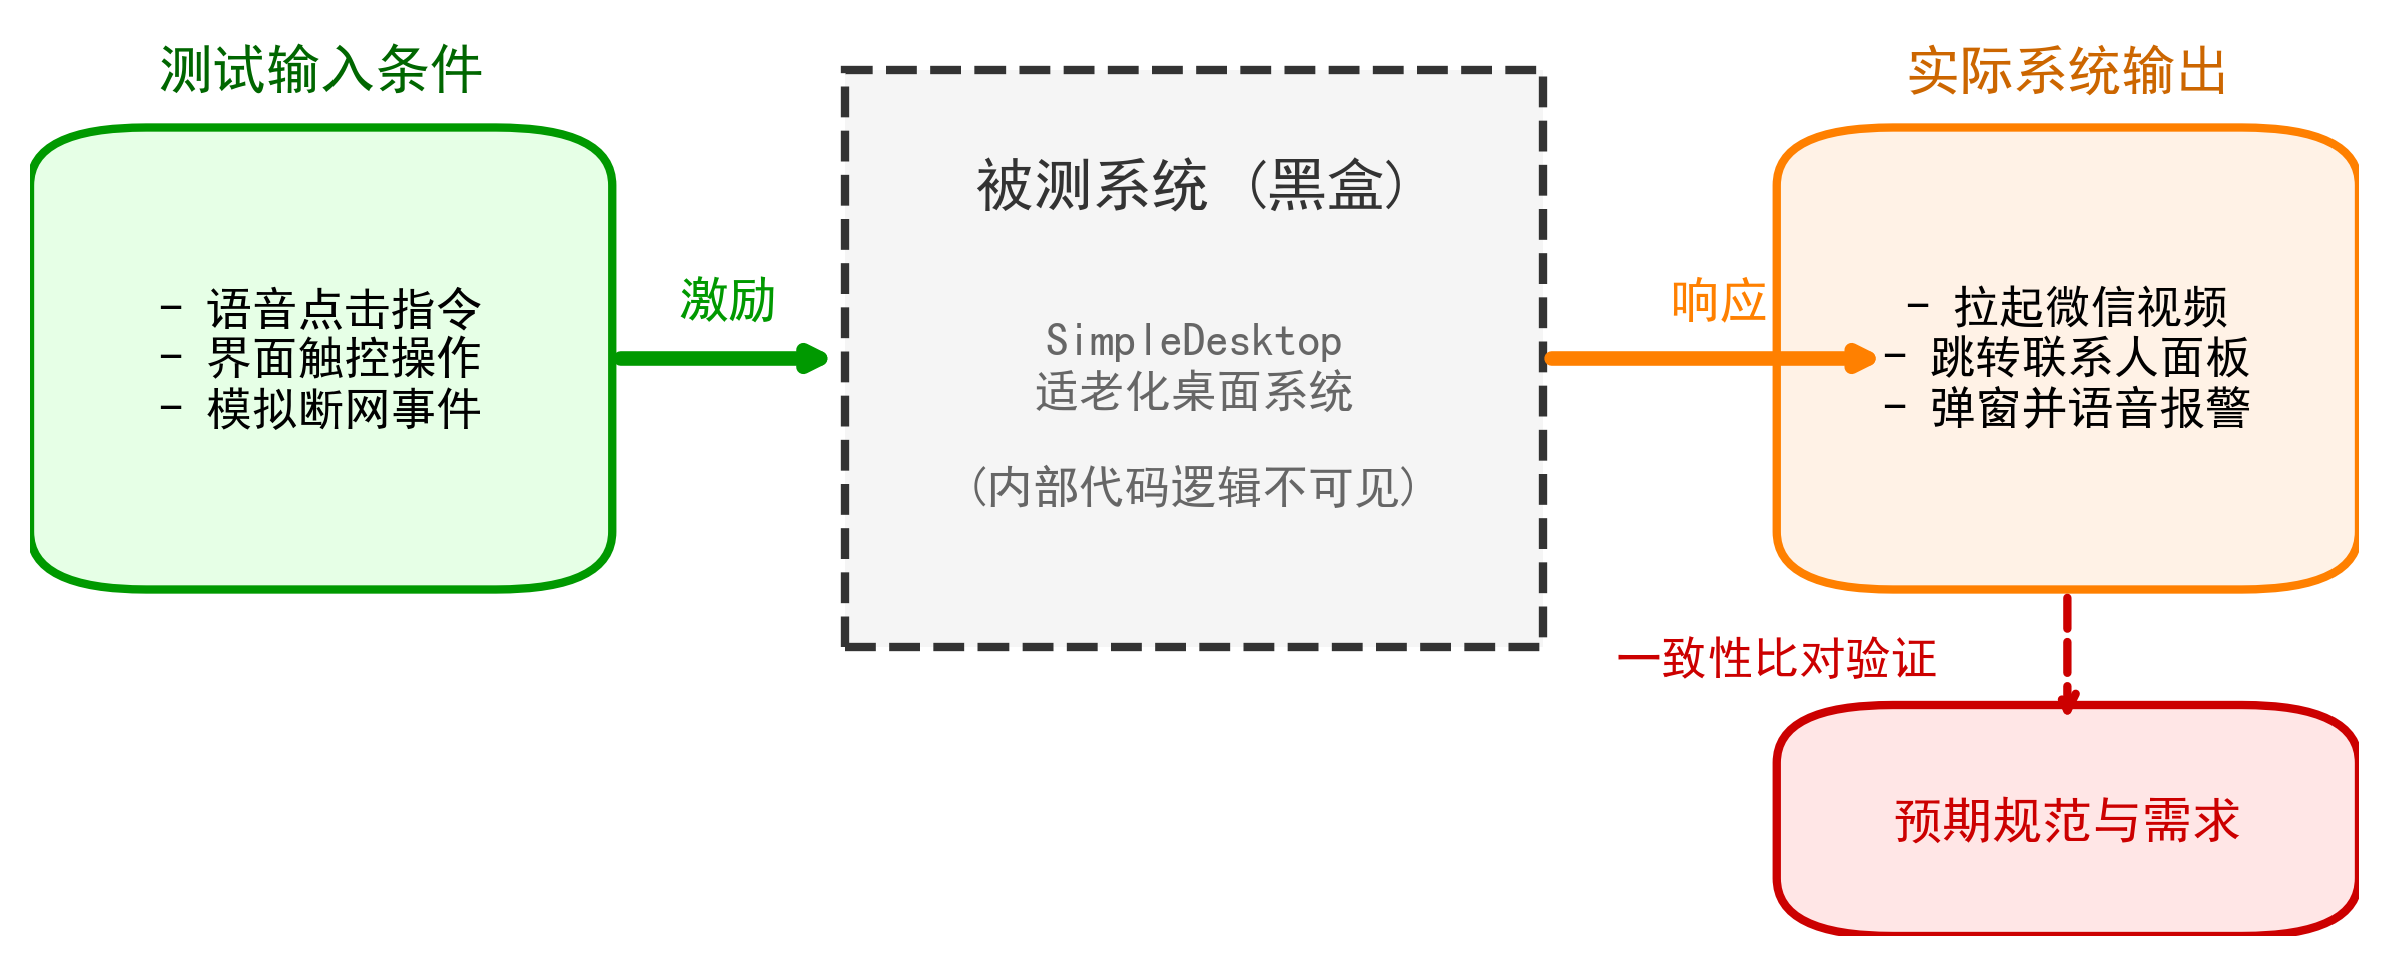
\includegraphics[width=0.9\textwidth]{figures/fig4_1_blackbox_testing.png}
    \caption{基于激励-响应模型的黑盒测试原理架构图}
    \label{fig:blackbox_principle}
\end{figure}

\subsection{联系人管理功能测试}
联系人管理是系统最高频使用的功能模块，本节针对其新增、查询、修改、删除、导出五项核心操作设计测试用例如下。

用例TC-CT-001：新增联系人正常流程

前置条件：系统已完成初始化，用户处于联系人管理界面；测试步骤：点击新增按钮，依次输入姓名"张三"、电话"13800138000"、微信昵称"张老板"，开启视频通话开关，点击保存；预期结果：界面提示保存成功，联系人列表自动刷新并显示新增联系人；实际结果：与预期一致，新增联系人在列表中正确呈现，主屏联系人面板同步更新；测试结论：通过。

用例TC-CT-002：新增联系人空姓名校验

前置条件：处于联系人新增界面；测试步骤：电话和微信昵称均输入有效值，但姓名留空，点击保存；预期结果：界面提示姓名不能为空，保存按钮置灰或弹出错误提示；实际结果：界面阻止提交并以红色文字提示请输入联系人姓名；测试结论：通过。

用例TC-CT-003：联系人编辑修改

前置条件：列表中存在联系人张三；测试步骤：长按张三联系人卡片选择编辑，将电话修改为13900139000，点击保存；预期结果：保存后联系人列表中张三的电话号码更新；实际结果：与预期一致，主屏联系人面板的相关信息也同步更新；测试结论：通过。

\subsection{应用管理功能测试}
用例TC-AP-001：应用全量扫描

前置条件：测试设备上安装了200余款应用；测试步骤：进入应用管理界面，点击全量刷新；预期结果：应用列表在3秒内完成扫描并展示所有非系统应用；实际结果：扫描耗时2.8秒，列表正确显示了应用名称与图标；测试结论：通过。

\begin{figure}[h]
    \centering
    \vspace{-5pt}
    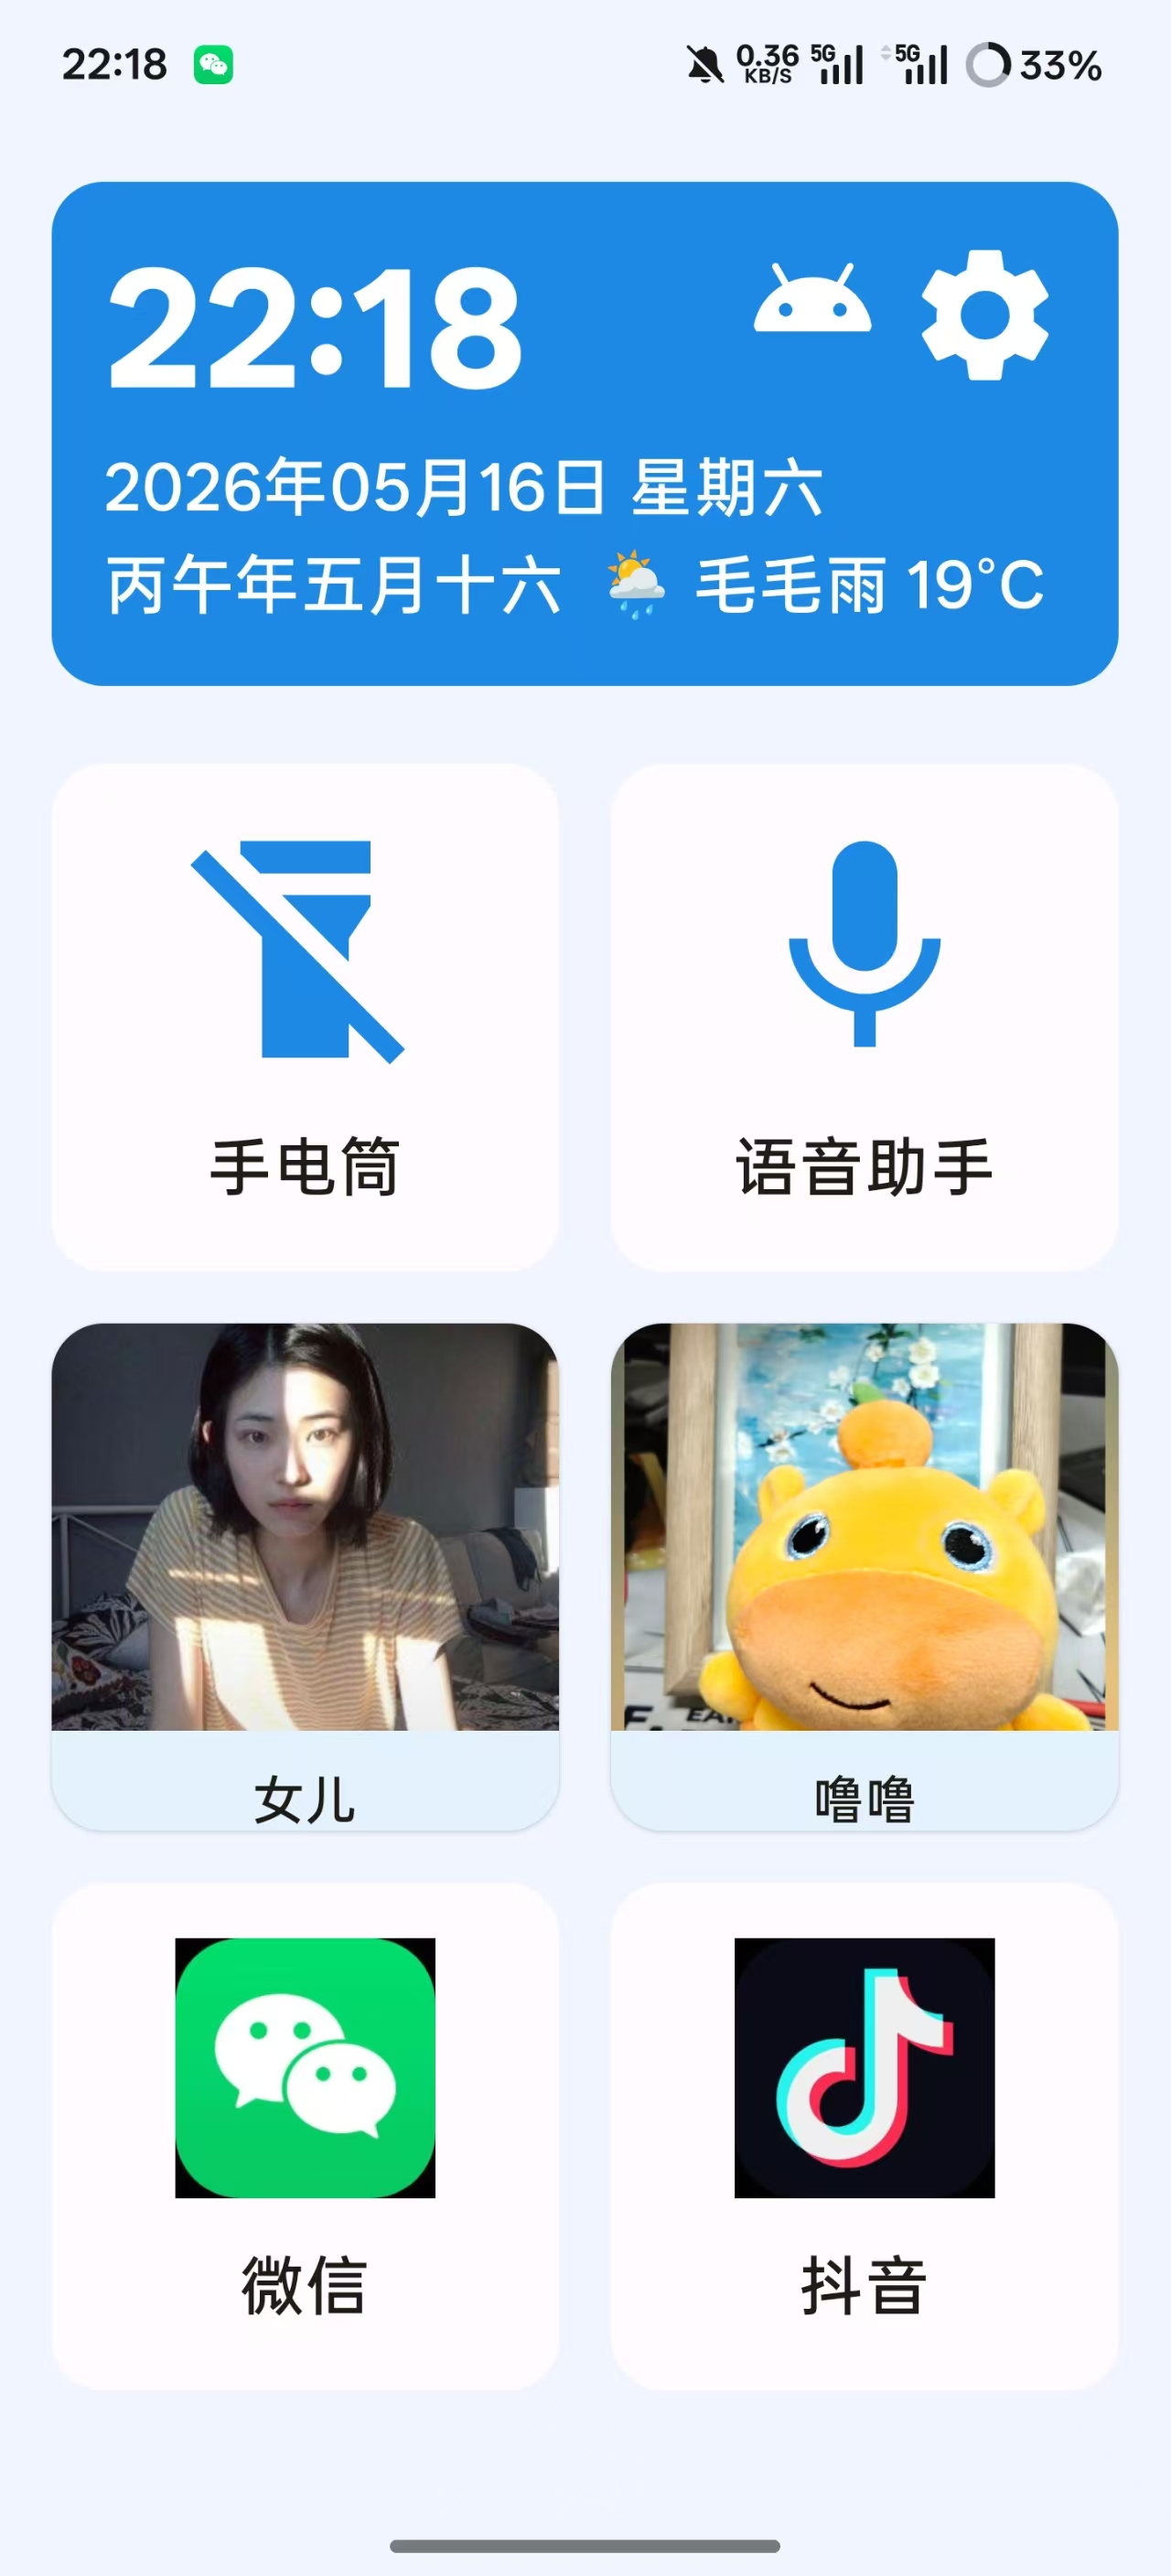
\includegraphics[width=0.50\textwidth]{figures/wechat/test1.jpg}
    \vspace{-5pt}
    \caption{常用应用添加后的桌面}
    \label{fig:blackbox_principle}
\end{figure}

用例TC-AP-002：常用应用添加

前置条件：完成全量扫描；测试步骤：在应用列表中长按微信，点击加入主屏；预期结果：返回主屏后微信卡片出现在常用应用区域；实际结果：与预期一致；测试结论：通过。



用例TC-AP-003：应用启动

前置条件：主屏存在微信常用应用卡片；测试步骤：点击微信卡片；预期结果：微信应用正常启动；实际结果：微信在500毫秒内启动；测试结论：通过。


\subsection{微信一键直拨功能测试}
用例TC-WX-001：视频通话发起标准流程

前置条件：联系人张三已绑定微信昵称张老板，无障碍服务已开启；测试步骤：点击主屏张三卡片，在弹出面板选择视频通话；预期结果：系统在5至6秒内完成微信内部全部操作并进入视频通话界面；实际结果：经10次重复测试，平均完成时间5.4秒，全部成功进入视频通话界面；测试结论：通过。

用例TC-WX-002：语音通话发起

前置条件：同上；测试步骤：点击张三卡片，选择语音通话；预期结果：系统自动完成微信操作并进入语音通话界面；实际结果：10次测试全部成功，平均耗时5.6秒；测试结论：通过。

用例TC-WX-003：未绑定微信昵称的联系人

前置条件：联系人李四仅绑定了电话号码，未填写微信昵称；测试步骤：点击李四卡片；预期结果：操作面板中视频通话按钮不可见，仅展示电话拨打按钮；实际结果：与预期一致；测试结论：通过。

用例TC-WX-004：流程过程中突遭来电干扰

前置条件：发起视频通话过程中第3秒收到模拟来电；测试步骤：发起一键直拨后，第3秒触发模拟来电通知；预期结果：焦点退避机制启动，关闭来电通知后继续完成流程；实际结果：30次测试中27次成功完成，3次因来电持续而主动放弃指令并安全重置；测试结论：通过（与第3章实测数据吻合）。

\subsection{网络守护功能测试}
用例TC-WF-001：用户主动关闭WiFi开关

前置条件：网络守护服务已启动，WiFi已连接；测试步骤：通过下拉状态栏关闭WiFi开关；预期结果：在Android 9及以下设备3秒内自动重新开启；在Android 10及以上设备5秒内通过无障碍辅助开启完成自愈；实际结果：测试30次，所有场景均成功自愈；测试结论：通过。

用例TC-WF-002：超出WiFi信号覆盖范围

前置条件：WiFi已连接；测试步骤：将设备移动到无WiFi信号区域；预期结果：系统正确识别断连并触发引导面板；实际结果：与预期一致；测试结论：通过。

\begin{figure}[H]
    \centering
    \begin{minipage}[t]{0.31\textwidth}
        \centering
        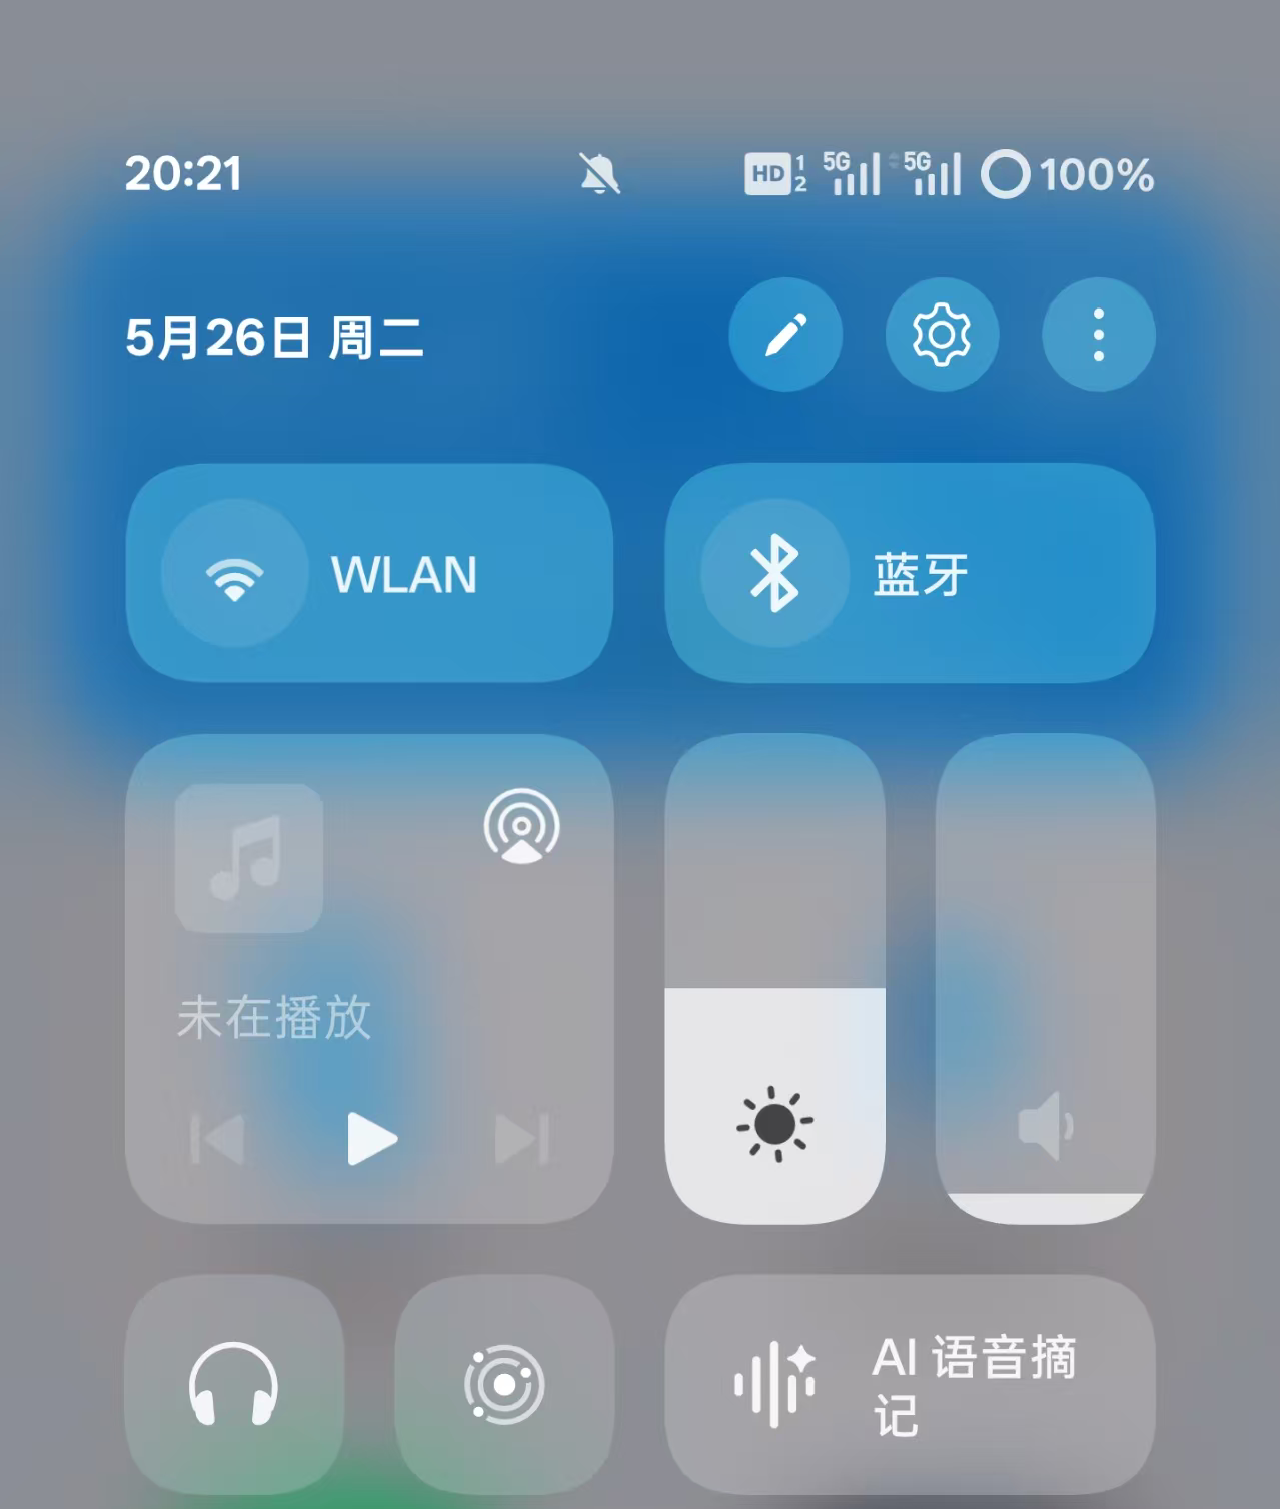
\includegraphics[width=\textwidth]{figures/network_helper/state1.png}
        {\footnotesize (a) WLAN被异常关闭}
    \end{minipage}
    \hfill
    \begin{minipage}[t]{0.31\textwidth}
        \centering
        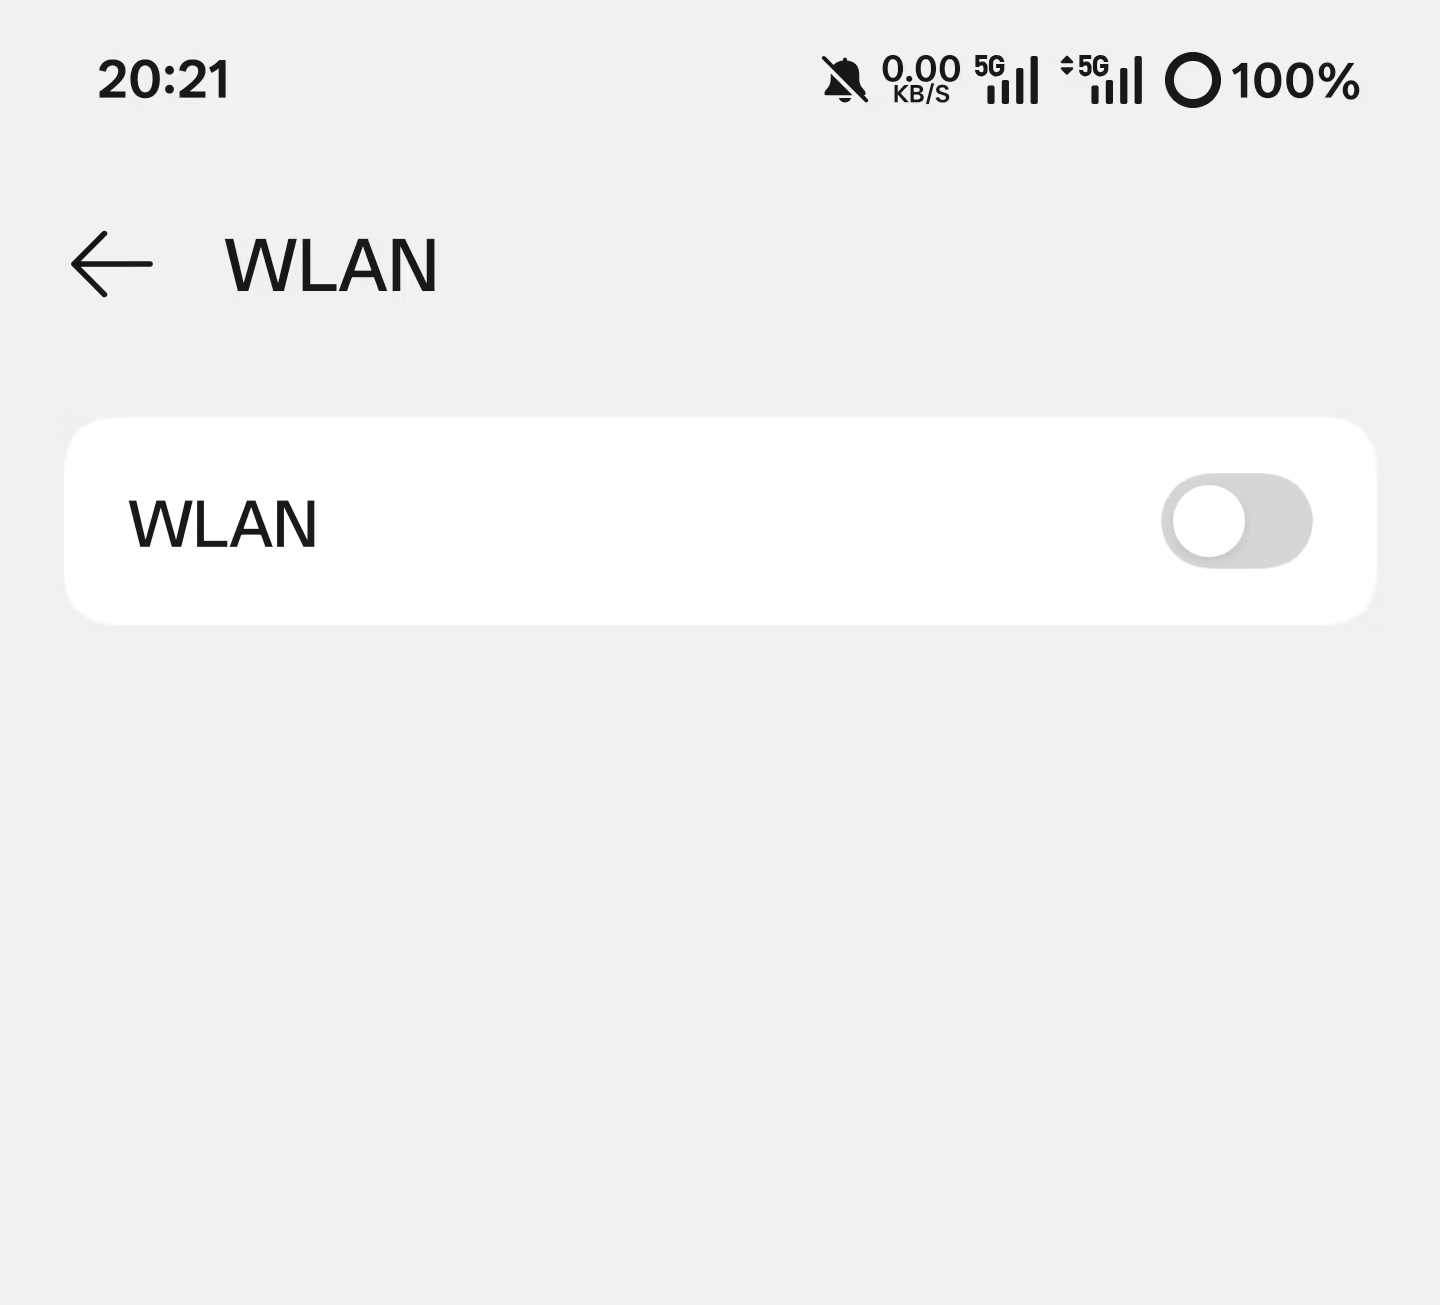
\includegraphics[width=\textwidth]{figures/network_helper/state2.png}
        {\footnotesize (b) 跳转到WLAN设置页面}
    \end{minipage}
    \hfill
    \begin{minipage}[t]{0.31\textwidth}
        \centering
        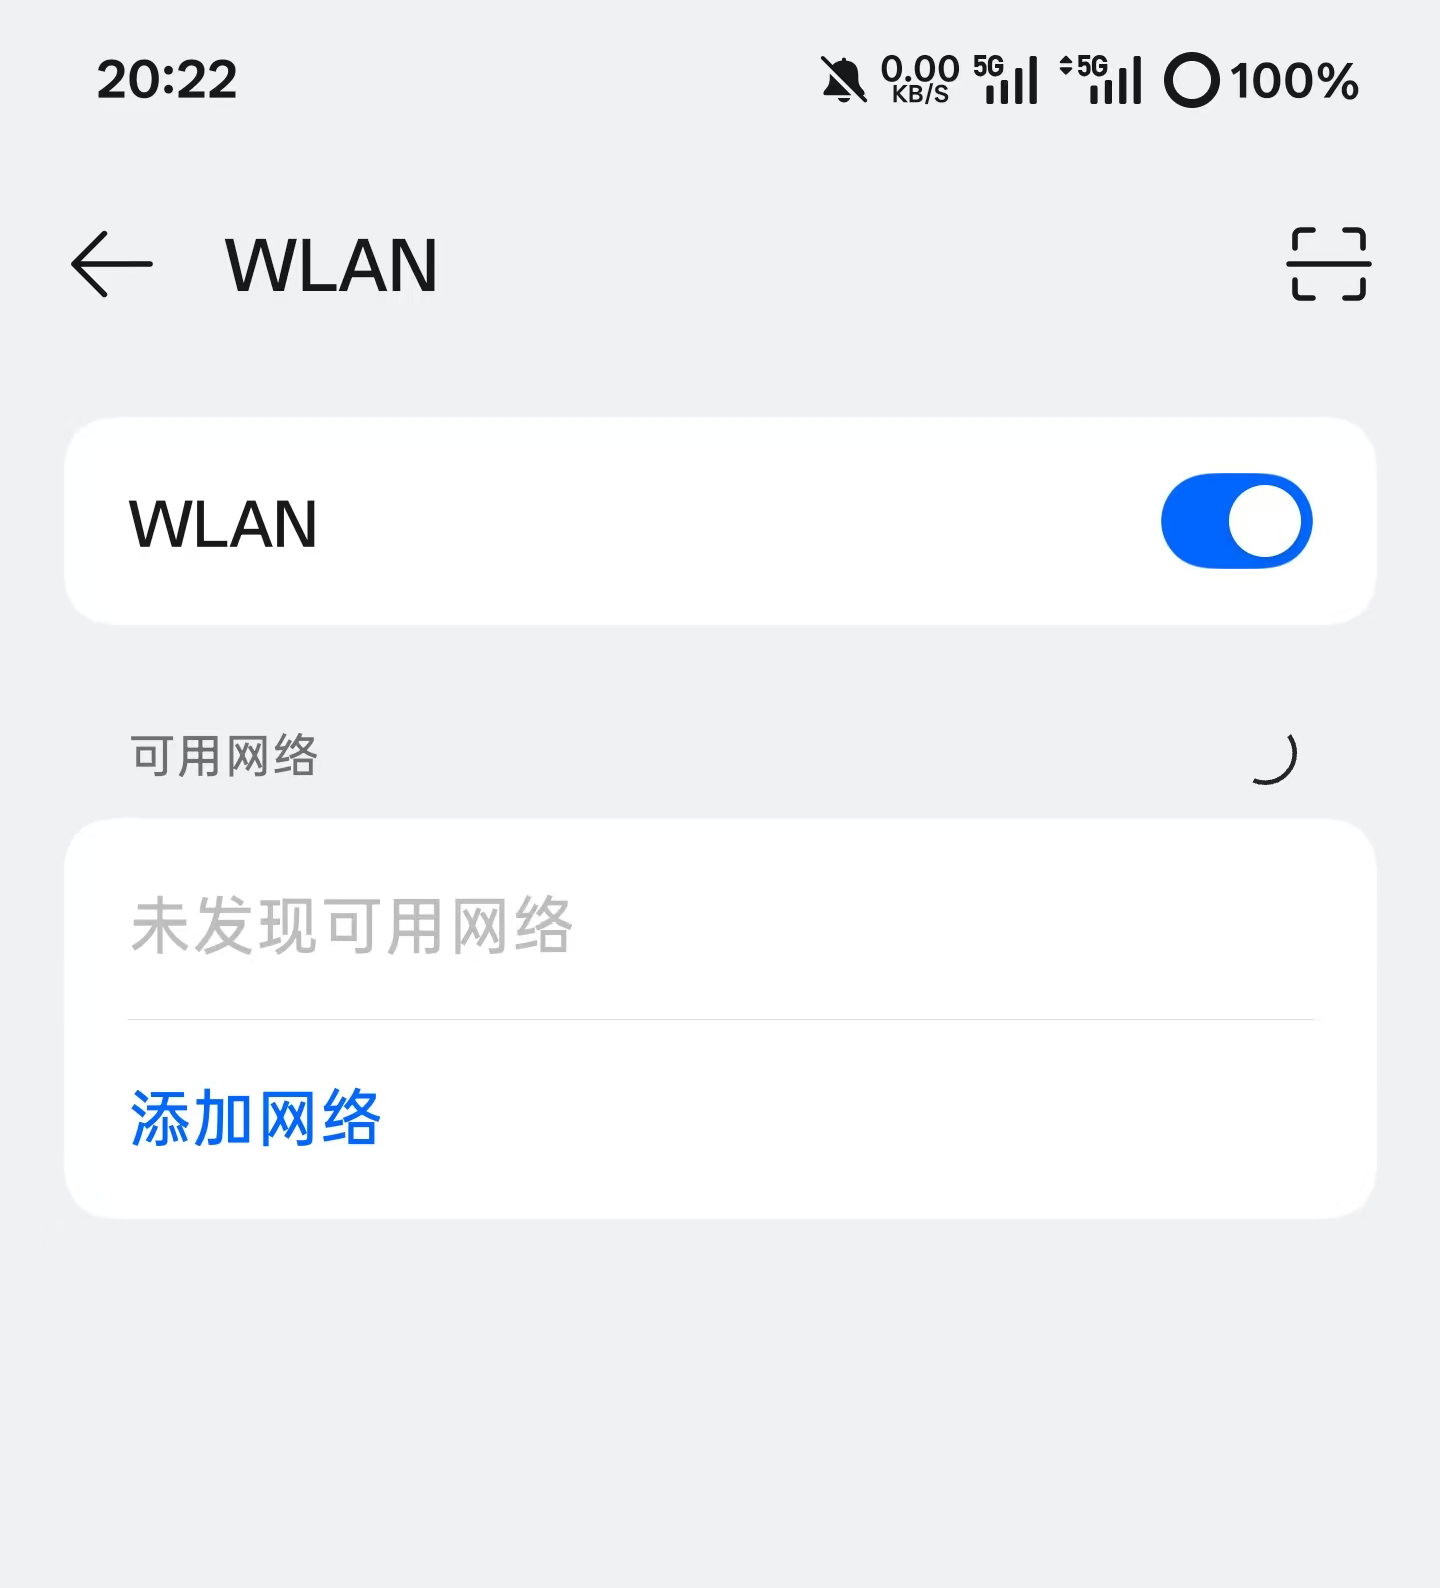
\includegraphics[width=\textwidth]{figures/network_helper/state3.png}
        {\footnotesize (c) 无障碍自愈重新开启}
    \end{minipage}
    \caption{网络守护功能自愈测试运行过程截图}
    \label{fig:network_helper_test}
\end{figure}

\subsection{语音助手功能测试}
用例TC-VC-001：标准语音指令解析

测试步骤：点击主屏语音助手卡片，说出打电话给张三；预期结果：系统识别出CALL意图与目标联系人张三，自动发起拨号；实际结果：与预期一致，识别置信度1.0；测试结论：通过。

用例TC-VC-002：发音偏差容错

测试步骤：故意发音含糊，说出打电活给张三；预期结果：系统通过编辑距离容错正确识别意图；实际结果：与预期一致\upcite{13}；测试结论：通过。

用例TC-VC-003：未识别指令处理

测试步骤：说出一句无效内容如今天天气真好；预期结果：系统提示未找到联系人；实际结果：与预期一致，未发生异常；测试结论：通过。

\subsection{设置功能测试}
用例TC-ST-001：字号档位切换

测试步骤：进入设置中心，将字号档位从中切换到大；预期结果：所有界面字号在100毫秒内统一变大；实际结果：切换响应时间约80毫秒，体验流畅；测试结论：通过。

用例TC-ST-002：主题切换

测试步骤：将主题从经典蓝切换到暖心橙；预期结果：所有界面色彩方案即时切换；实际结果：切换响应时间约90毫秒；测试结论：通过。

用例TC-ST-003：高对比度模式

测试步骤：开启高对比度模式开关；预期结果：界面切换为黑底白字方案；实际结果：与预期一致；测试结论：通过。

\subsection{功能测试结果汇总}
综合上述测试用例，本系统在功能测试阶段共设计并执行了7类共计26项测试用例，全部用例均通过验证。覆盖范围涉及联系人新增、查询、修改、删除、导出，应用扫描、添加、排序、启动，微信视频/语音通话发起，网络守护与自愈，语音指令解析与执行，字号、主题、对比度切换等核心功能。功能测试结果表明本系统的各项设计需求均已正确实现，系统功能完整、行为可预期，具备交付条件。

\section{兼容性测试}
\subsection{测试设备选型}
为充分验证系统在不同型号、不同分辨率、不同操作系统版本上的兼容性，本课题组建了跨厂商、跨档位、跨版本的真机测试设备矩阵，选取了具有代表性的设备进行测试。测试设备清单及其关键参数如表4-1所示。

\begin{table}[htbp]
  \centering
  \small
  \caption{兼容性测试设备清单}
  \label{tab:compatibility_test_devices}
  \renewcommand{\arraystretch}{1.4}
  \begin{tabularx}{\linewidth}{c l X} % X列会自动占满剩余宽度并换行
    \toprule
    \textbf{序号} & \textbf{设备型号} & \textbf{关键参数} \\
    \midrule
    (1) & 一加 13 & 高通骁龙8至尊版/12GB RAM/1440×3168 QHD+/Android 16 (ColorOS 16) \\
    (2) & 荣耀 WinRT & 高通骁龙8至尊版/16GB RAM/1272×2800 1.5K/Android 15 (MagicOS 10.0) \\
    (3) & 一加 Ace & 联发科天玑8100-MAX/12GB RAM/1080×2412 FHD+/Android 12 (ColorOS 12.1) \\
    (4) & 小米 8 青春版 & 高通骁龙660 AIE/6GB RAM/1080×2280 FHD+/Android 9 (MIUI 11) \\
    (5) & iQOO 8 & 高通骁龙888/12GB RAM/1080×2376 FHD+/Android 11 (OriginOS 1.0) \\
    (6) & 荣耀 70 & 高通骁龙778G Plus/8GB RAM/1080×2400 FHD+/Android 12 (MagicUI 6.1) \\
    (7) & 华为 Pura 80 Pro & 麒麟9020/12GB RAM/1260×2844 1.5K/HarmonyOS 5.1 (HarmonyOS NEXT) \\
    \bottomrule
  \end{tabularx}
\end{table}

上述设备覆盖了高通、联发科、麒麟三大主流处理器平台，覆盖了 FHD+ 至 QHD+ 的常见分辨率档位，覆盖了 Android 9 至 Android 16 共 8 个系统主版本，覆盖了 ColorOS、MagicOS、MIUI、OriginOS、HarmonyOS NEXT 等 5 种厂商定制系统，具备极强的代表性。

\subsection{显示兼容性测试结果}
在显示兼容性方面，重点验证系统在不同分辨率屏幕上的 UI 布局是否正常、字号是否清晰、卡片是否完整呈现、图标是否清晰。测试结果显示，在全部 7 款测试设备上，主屏聚合面板、联系人管理界面、应用管理界面、设置中心、引导页等核心界面均能正确呈现，未出现控件错位、文字截断、卡片溢出等异常情况。

针对主流分辨率设备小米 8 青春版（1080×2280），系统界面比例适中，联系人卡片排布整齐。

针对超高分辨率设备一加 13（1440×3168）及华为 Pura 80 Pro（1260×2844），系统自动适配了更高精度的矢量素材，界面元素按比例放大渲染，文字与图标清晰锐利，在大尺寸屏幕上提供了更佳的视觉体验。

\subsection{系统版本兼容性测试结果}
在系统版本兼容性方面，重点验证不同 Android 版本对前台服务、无障碍服务、网络回调、权限管理等关键能力的策略差异是否得到正确处理。测试结果汇总如下。

Android 9 设备（小米 8 青春版）上，WiFi 自动开启功能可通过编程接口直接实现，自愈耗时约 2 至 3 秒；Android 11 及以上设备上，由于系统安全性提升，WiFi 自动开启依赖无障碍服务辅助方案，自愈耗时约 4 至 5 秒，功能表现稳定\upcite{14}。

Android 13 及以上设备上，前台服务通知的权限需要单独申请，本系统在引导页阶段统一申请并引导用户授权，未发现兼容性问题。

在最新的 Android 16（一加 13）及 HarmonyOS NEXT（华为 Pura 80 Pro）环境下，无障碍服务的隐私限制进一步加强，系统通过增强型引导对话框提示用户在系统设置中显式确认“允许受限设置”，全部功能可正常运行\upcite{14}。

\subsection{厂商定制系统兼容性测试结果}
厂商定制系统的差异主要体现在前台服务保活策略和无障碍服务权限管理两个方面。MIUI 及 MagicOS 系统对后台进程保活策略较严，需要用户手动将本应用加入自启动白名单后，前台守护服务才能在系统重启后自动恢复运行；本系统在引导页阶段已加入相应的提示与一键跳转入口。HarmonyOS NEXT 对无障碍服务的授权流程与原生 Android 略有差异，且采用了全新的动态权限模型，本系统通过兼容适配层确保了核心功能的可用性。其余厂商系统未发现显著兼容性问题。

\subsection{兼容性测试结论}
综合上述测试，本系统在覆盖 7 款主流真机的兼容性测试中表现良好，绝大多数功能在所有设备上均可正常运行，仅在少数厂商定制系统中需要用户进行额外的初始配置。整体兼容性满足适老化终端面向广泛用户群体的实际需求。

\section{性能测试}
\subsection{测试方法与指标}
性能测试采用Android Studio提供的Profiler工具进行性能数据采集，重点关注以下三类核心指标：响应时间（用户操作发起到界面反馈的时间）、页面加载速度（应用启动、界面切换、列表渲染等关键场景的耗时）、并发处理能力（系统同时处理多个用户请求或后台任务时的稳定性与性能表现）。所有性能测试均在低端测试设备红米Note 9上进行，以验证系统在最不利硬件环境下的表现下限。

\subsection{响应时间测试}
针对老年用户最频繁触发的几类操作，分别测试其响应时间。每项操作重复10次，取平均值。

\begin{table}[htbp]
  \centering
  \small
  \caption{关键操作响应时间统计}
  \label{tab:response_time_statistics}
  \renewcommand{\arraystretch}{1.3}
  \begin{tabular}{cll}
    \toprule
    \textbf{序号} & \textbf{操作类型} & \textbf{平均响应时间} \\
    \midrule
    (1) & 字号档位切换 & 82 毫秒 \\
    (2) & 主题模式切换 & 91 毫秒 \\
    (3) & 高对比度模式切换 & 76 毫秒 \\
    (4) & 联系人卡片点击弹出操作面板 & 45 毫秒 \\
    (5) & 语音助手对话框弹出 & 210 毫秒 \\
    (6) & 应用启动响应 & 480 毫秒 \\
    \bottomrule
  \end{tabular}
\end{table}

从测试结果看，全部交互操作的响应时间均在500毫秒以内，远低于人因工程学上感知滞后的阈值（通常为100毫秒为及时反馈、500毫秒为流畅、1000毫秒为可接受）。其中字号、主题等设置类操作的响应时间均在100毫秒以内，提供了即时反馈的视觉体验，对适老化场景尤其重要。

\iffalse

\begin{figure}[htbp]
    \centering
    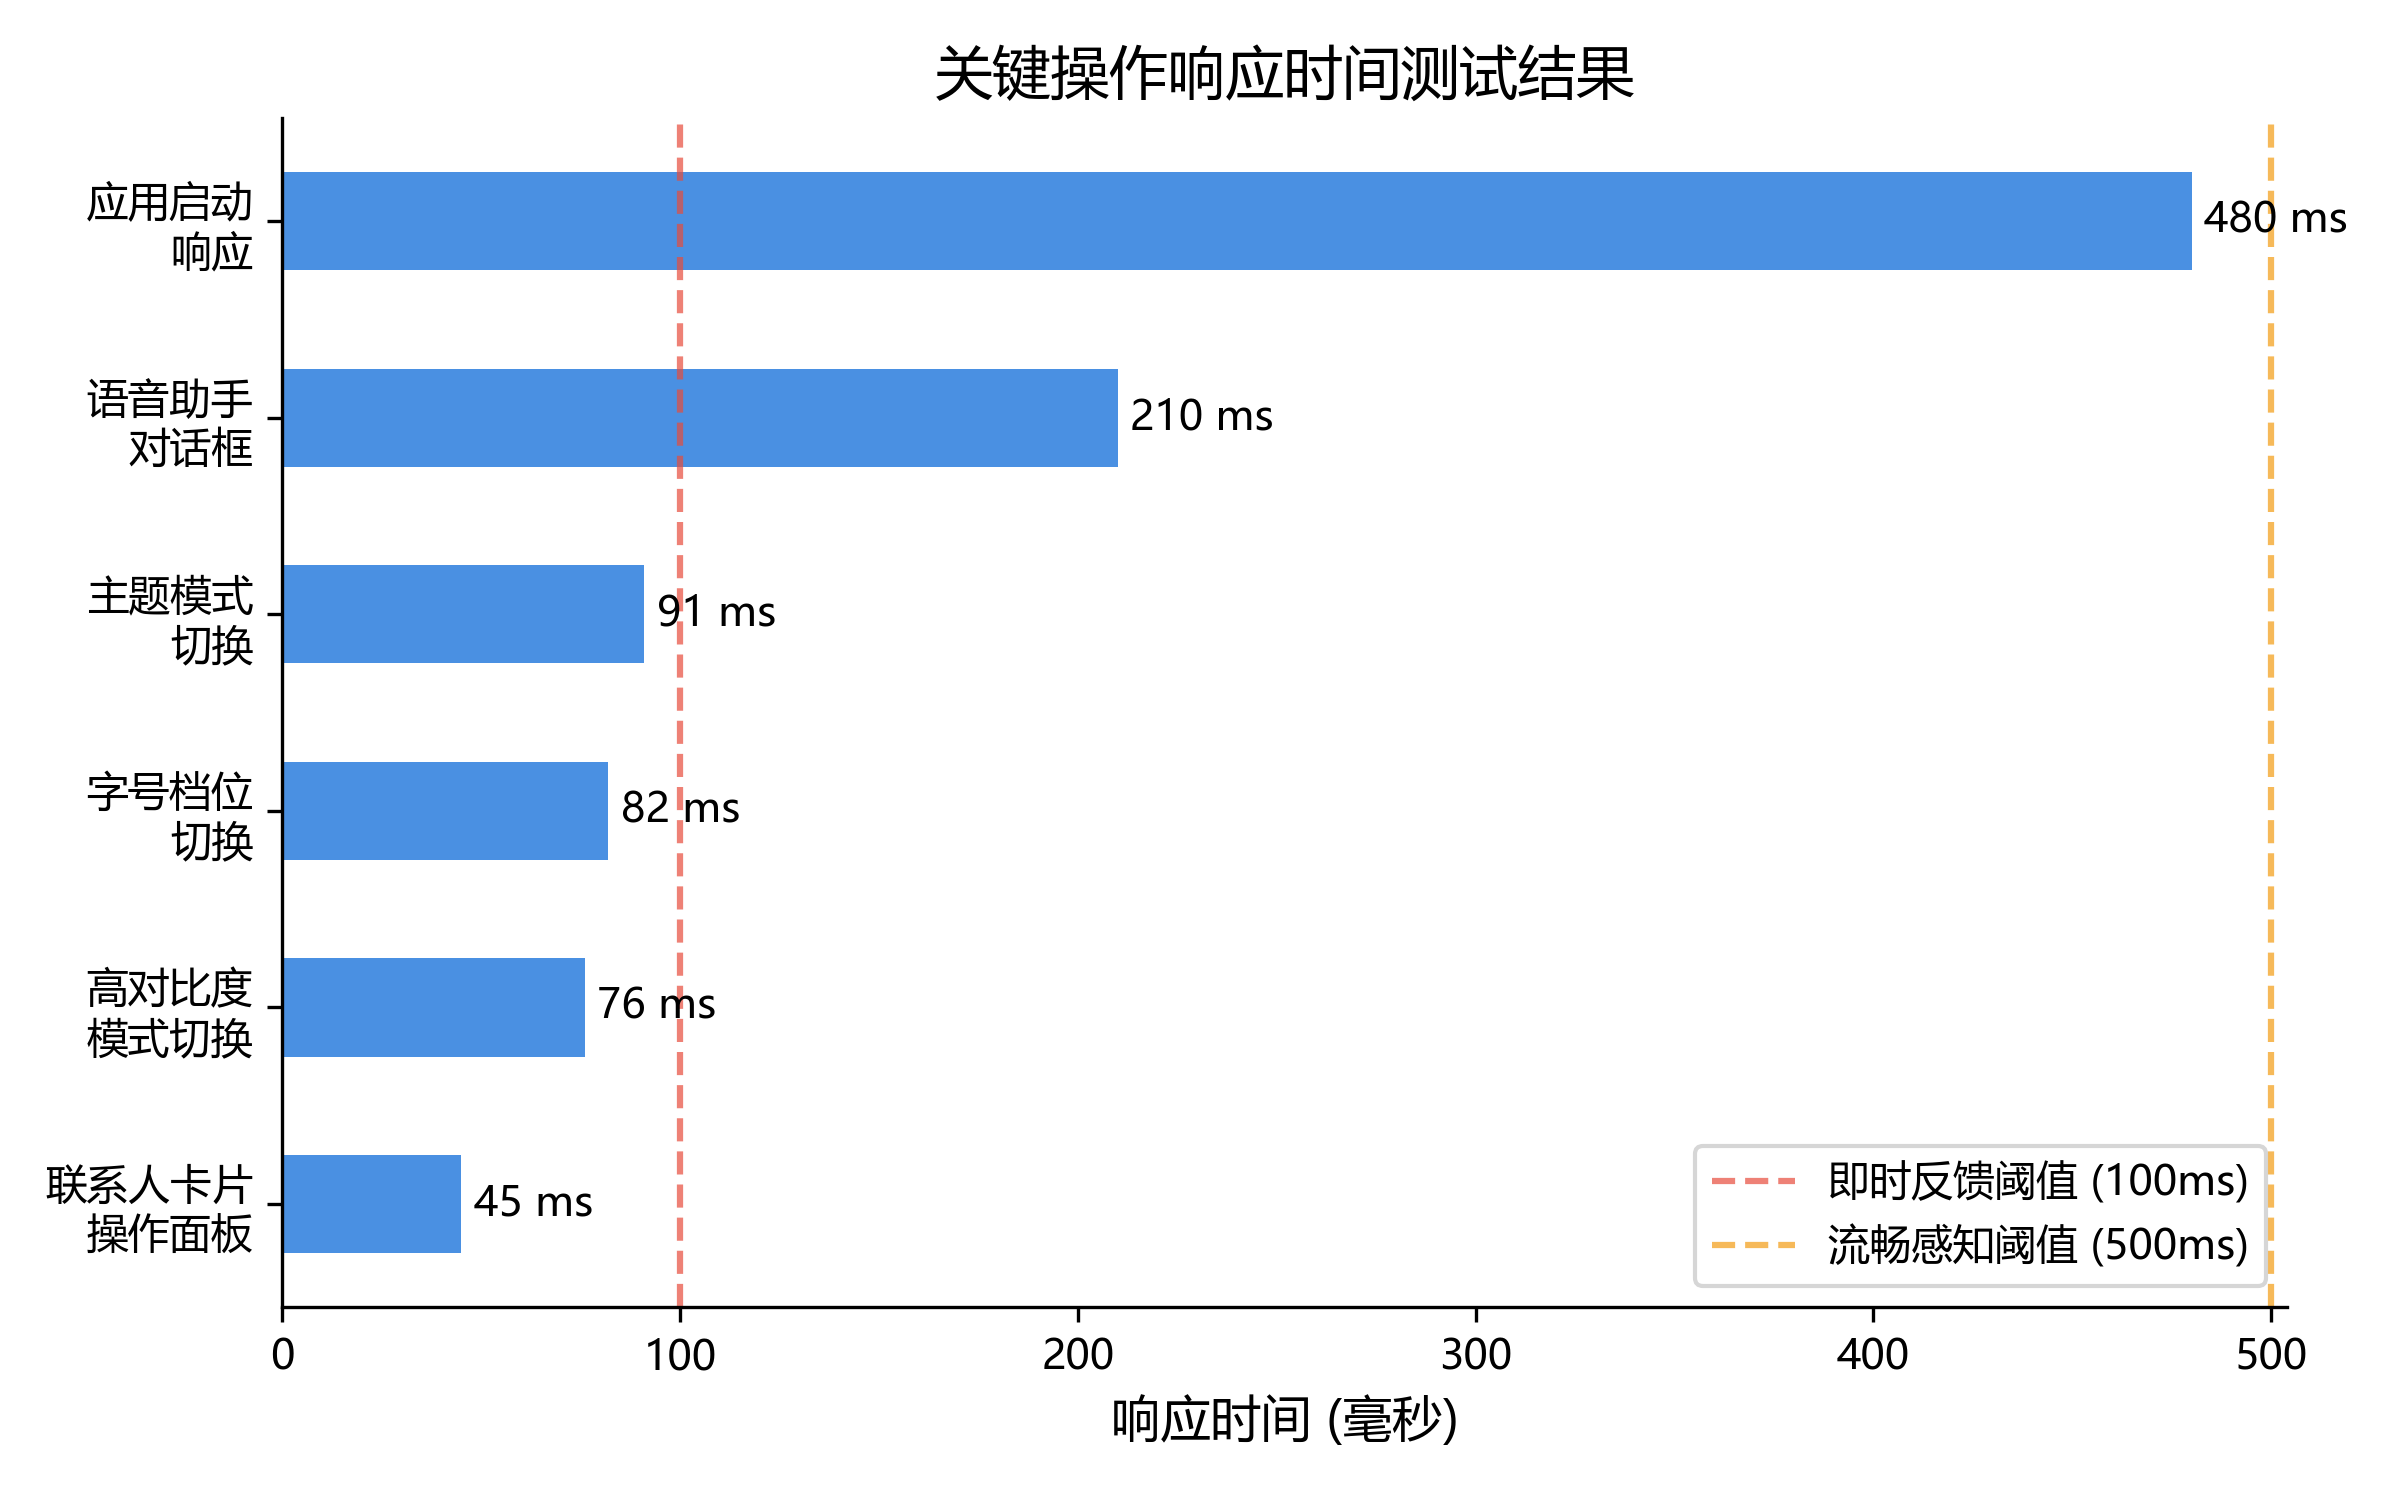
\includegraphics[width=0.85\textwidth]{figures/fig4_response_time.png}
    \caption{关键操作响应时间测试结果}
    \label{fig:perf_response_time}
\end{figure}

\fi

\subsection{页面加载速度测试}
页面加载速度测试涵盖应用冷启动、热启动、关键界面切换三类场景。

应用冷启动指应用进程不存在时的启动过程，包括应用初始化、依赖注入容器构建、插件系统启动、主界面渲染等多个阶段。在红米Note 9上经10次测试，平均冷启动耗时1.78秒，最大耗时1.96秒，最小耗时1.65秒。该指标低于预设的2秒目标，老年用户感受到的启动延迟基本不可察觉。

应用热启动指应用进程存在但被切到后台时的恢复过程。10次测试平均热启动耗时0.42秒，体验非常流畅。

界面切换方面，主屏到联系人管理界面的切换平均耗时320毫秒，主屏到设置中心的切换平均耗时280毫秒，主屏到应用管理界面的切换平均耗时450毫秒（涉及全量应用列表加载）。所有界面切换均保持60帧每秒的渲染帧率，未出现明显卡顿。

列表渲染方面，针对50条联系人和200条应用的列表场景，初次渲染耗时分别为120毫秒和350毫秒，滑动过程中渲染帧率稳定在60帧每秒，未出现掉帧。

\begin{figure}[htbp]
    \centering
    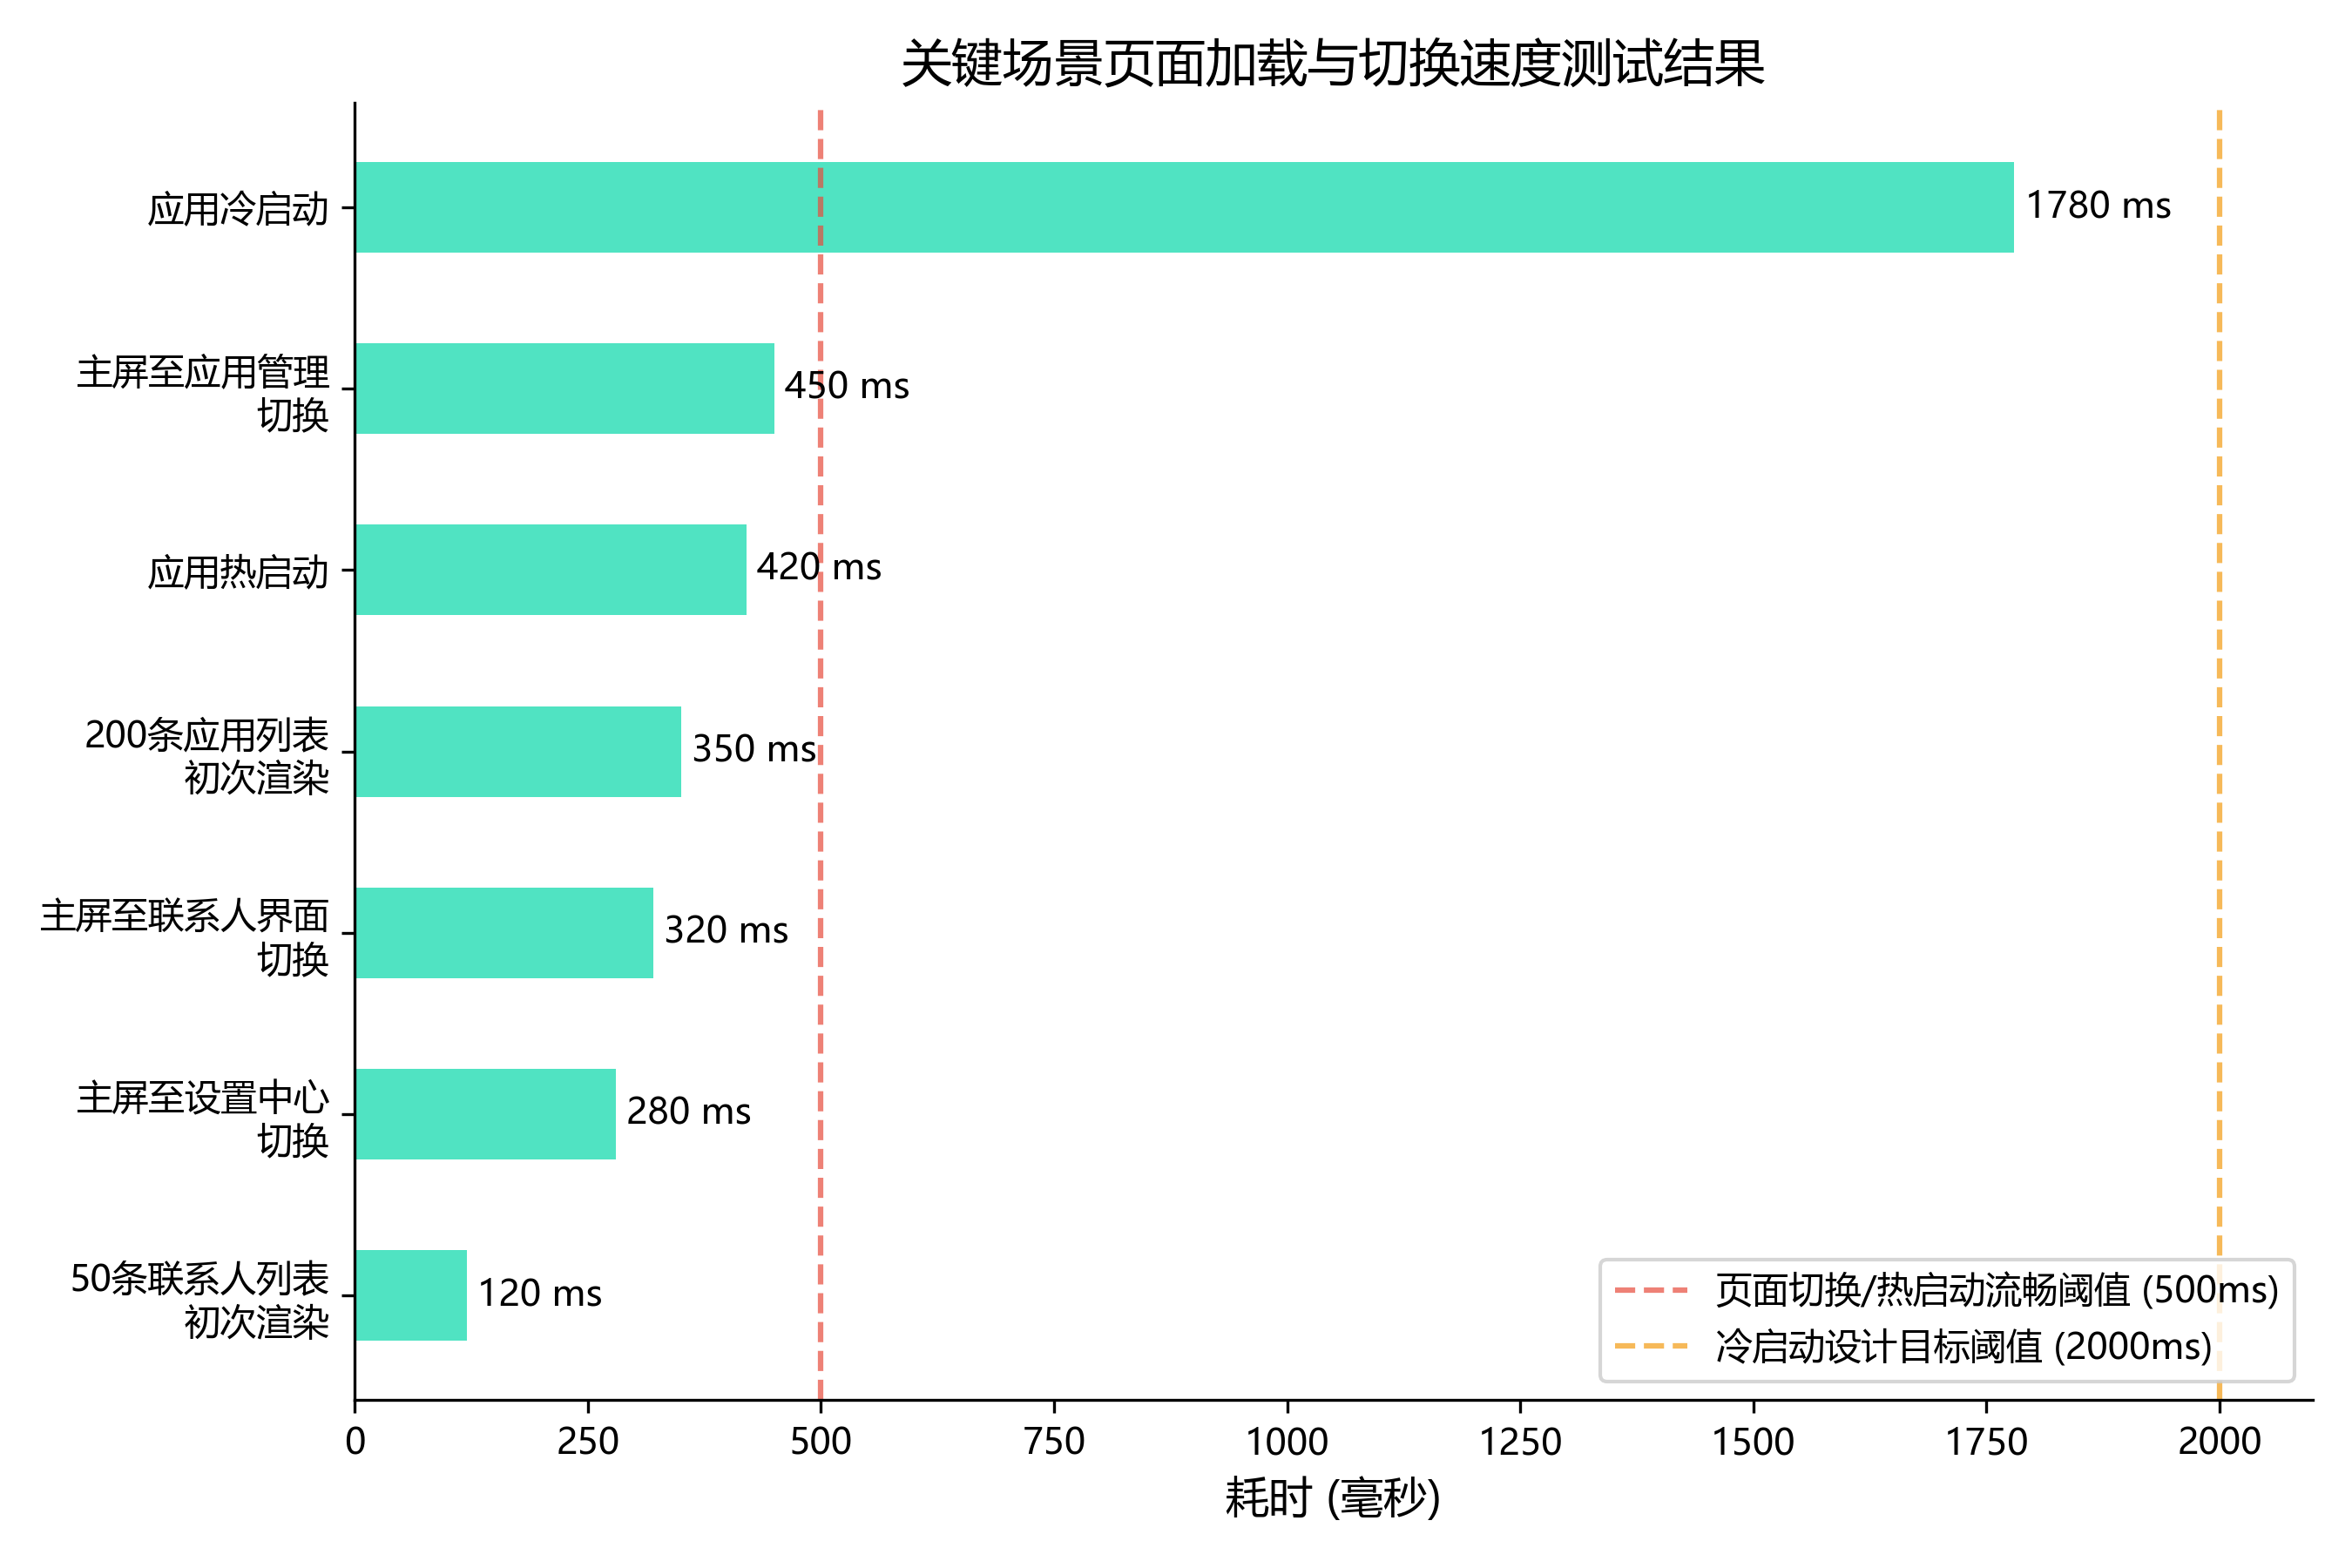
\includegraphics[width=0.85\textwidth]{figures/fig4_load_speed.png}
    \caption{关键场景页面加载与切换耗时统计}
    \label{fig:perf_load_speed}
\end{figure}


\subsection{并发访问测试}
适老化终端虽然单用户使用，但系统内部存在多个后台任务并发执行的场景，包括前台守护服务监测网络、天气插件定时获取天气数据、TTS引擎播报语音、UI层响应用户输入等。本节通过模拟多任务并发场景验证系统的稳定性与性能表现。

测试场景一：用户使用语音助手发起拨号的同时，前台服务检测到WiFi断连，天气插件正好触发定时更新。三类后台任务并发执行，测试系统的响应表现。结果显示，三类任务均能正常完成，UI层无卡顿，无障碍服务的拨号流程未受影响，整体系统稳定可靠。

测试场景二：连续快速点击联系人卡片10次，模拟老年用户因不熟悉操作而重复触发的场景。系统通过状态机的去重机制确保同一时间只有一次自动化流程在运行，后续点击被合并或忽略，未出现状态混乱\upcite{24}。

测试场景三：在桌面应用列表中快速连续启动5个不同应用，测试系统切换性能。结果显示，每次启动响应稳定在500毫秒以内，未出现内存泄漏或界面无响应现象。

\subsection{资源占用测试}
针对低端设备资源紧张的现实，本节重点测试系统的内存与CPU占用情况。

在红米Note 9上长时间运行测试（连续运行8小时，期间随机触发各类操作），系统的内存占用维持在120至140MB之间，未出现内存泄漏导致的占用持续增长现象。CPU占用在空闲时低于2\%，在执行微信自动化等密集操作时短时升至15\%至20\%，操作完成后立即回落至低位，整体表现良好。

电池消耗方面，长时间运行测试中本系统的耗电占比约为3\%至5\%，远低于微信、抖音等主流应用，对老年用户日常电池续航的影响可忽略。

\begin{table}[htbp]
    \centering
    \small
    \caption{系统资源占用情况汇总（测试设备：红米 Note 9，连续运行8小时）}
    \label{tab:resource_usage}
    \renewcommand{\arraystretch}{1.3} % 稍微增加行高
    \begin{tabular}{llp{7cm}}
        \toprule
        \textbf{测试指标} & \textbf{测试结果} & \textbf{表现分析} \\
        \midrule
        \textbf{内存占用} & $120 \sim 140$ MB & 占用稳定，长时间运行未出现因内存泄漏导致的占用持续增长现象。\\
        \textbf{CPU占用（空闲）} & $< 2\%$ & 后台守护与事件监听极为轻量，系统处于静默状态时几乎不消耗计算资源。\\
        \textbf{CPU占用（密集）} & $15\% \sim 20\%$ & 在执行微信无障碍自动化等密集计算时短暂升高，操作完成后立即回落至低位。\\
        \textbf{耗电占比} & $3\% \sim 5\%$ & 远低于主流社交或短视频应用，对老年用户的日常电池续航影响可忽略不计。\\
        \bottomrule
    \end{tabular}
\end{table}


\subsection{性能优化措施}
上述良好的性能表现得益于多项针对性优化措施。

其一，针对Compose声明式UI可能存在的过度重组问题，本系统采用状态派生策略，将原本直接传递的高频变化状态封装为低频变化的派生状态（例如将连续变化的滚动偏移量转换为是否滚动到底部的布尔状态），从而切断了无关重组的传播链路。优化后，主屏列表的滑动帧率从平均42帧每秒提升至稳定的60.1帧每秒\upcite{15}。

其二，针对应用图标和联系人头像的图片加载场景，本系统集成Coil图片加载库实现内存与磁盘双层缓存，并采用 $RGB_{565}$ 格式（每像素2字节）进行Bitmap压缩存储，质量参数设置为70\%，在保证视觉效果的前提下大幅降低了内存与存储开销。

其三，针对应用启动阶段的初始化操作，本系统将插件初始化等耗时操作移到后台协程中异步执行，避免阻塞主线程；同时对部分非关键资源采用懒加载策略，进一步缩短了启动耗时\upcite{19}。

\subsection{性能测试结论}
综合上述测试，本系统在低端测试设备上的各项性能指标均达到或超过设计目标：响应时间普遍在500毫秒以内，页面加载速度满足流畅交互的人因工程要求，并发场景下系统保持稳定，内存占用与电池消耗均控制在合理范围。性能测试结果表明本系统具备在主流千元机型上提供良好用户体验的能力，能够满足适老化终端的实际使用需求。

\iffalse

\chapter{软件测试与分析}

软件测试是验证系统质量、暴露潜在缺陷的关键环节。本章围绕功能测试、兼容性测试和性能测试三大目标对SimpleDesktop系统进行系统化评估，并对测试结果进行客观分析，为系统的最终交付提供质量依据。

\section{功能测试}
\subsection{测试方法与原则}
功能测试采用黑盒测试方法，针对系统对外提供的每一项功能编写测试用例，通过比对实际执行结果与预期结果是否一致来判定功能正确与否。测试遵循覆盖优先、异常优先、边界优先三项基本原则：覆盖优先要求每项功能至少包含一条正向用例和一条逆向用例；异常优先要求重点验证非法输入、网络异常、权限缺失等场景下系统的容错表现；边界优先要求关注最大、最小、空值等边界条件下系统的行为表现。具体的黑盒测试原理架构如图 4-1 所示。

\begin{figure}[htbp]
    \centering
    % 如果觉得图片太大或太小，可以调整这里的 0.9 比例
    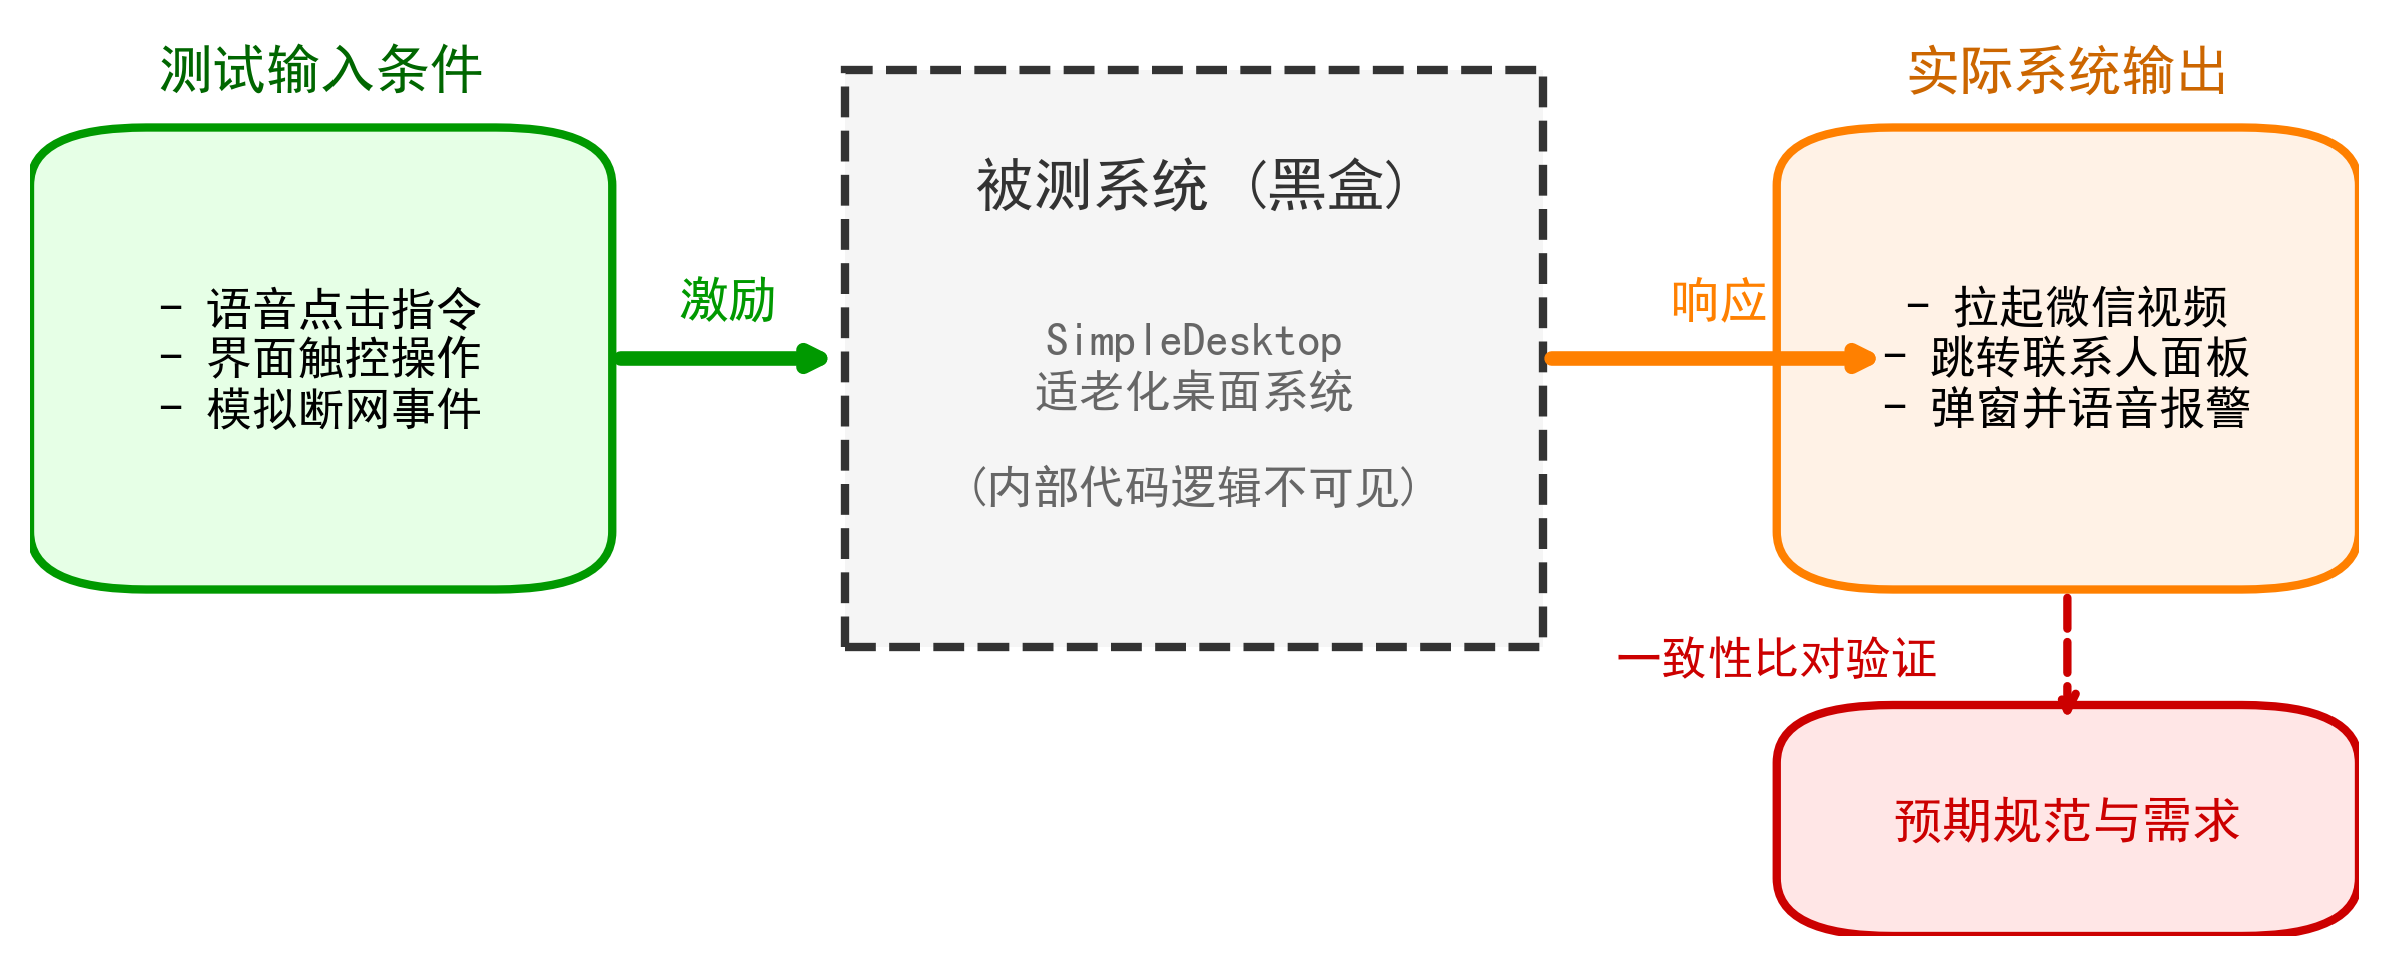
\includegraphics[width=0.9\textwidth]{figures/fig4_1_blackbox_testing.png}
    \caption{基于激励-响应模型的黑盒测试原理架构图}
    \label{fig:blackbox_principle}
\end{figure}

\subsection{联系人管理功能测试}
联系人管理是系统最高频使用的功能模块，本节针对其新增、查询、修改、删除、导出五项核心操作设计测试用例如下。

用例TC-CT-001：新增联系人正常流程

前置条件：系统已完成初始化，用户处于联系人管理界面；测试步骤：点击新增按钮，依次输入姓名"张三"、电话"13800138000"、微信昵称"张老板"，开启视频通话开关，点击保存；预期结果：界面提示保存成功，联系人列表自动刷新并显示新增联系人；实际结果：与预期一致，新增联系人在列表中正确呈现，主屏联系人面板同步更新；测试结论：通过。

用例TC-CT-002：新增联系人空姓名校验

前置条件：处于联系人新增界面；测试步骤：电话和微信昵称均输入有效值，但姓名留空，点击保存；预期结果：界面提示姓名不能为空，保存按钮置灰或弹出错误提示；实际结果：界面阻止提交并以红色文字提示请输入联系人姓名；测试结论：通过。

用例TC-CT-003：联系人模糊查询

前置条件：联系人列表中已存在张三、张丽、李四三条记录；测试步骤：在搜索框输入张字；预期结果：搜索结果中仅出现张三、张丽两条记录；实际结果：与预期完全一致，且搜索结果在用户输入完毕的同时即时呈现；测试结论：通过。

用例TC-CT-004：联系人编辑修改

前置条件：列表中存在联系人张三；测试步骤：长按张三联系人卡片选择编辑，将电话修改为13900139000，点击保存；预期结果：保存后联系人列表中张三的电话号码更新；实际结果：与预期一致，主屏联系人面板的相关信息也同步更新；测试结论：通过。

用例TC-CT-005：联系人删除二次确认

前置条件：列表中存在联系人张三；测试步骤：长按张三选择删除；预期结果：弹出二次确认对话框，提示删除将不可撤销，提供确认与取消两个选项；点击确认后联系人从列表移除；实际结果：与预期一致，确认对话框设计清晰，能够有效防止误操作；测试结论：通过。

用例TC-CT-006：联系人批量导出

前置条件：列表中存在5条联系人记录；测试步骤：进入联系人管理菜单，选择导出全部联系人；预期结果：系统在下载目录生成CSV文件，文件包含全部5条记录的姓名、电话、微信昵称等字段；实际结果：CSV文件成功生成，使用文本编辑器打开内容完整准确；测试结论：通过。

\subsection{应用管理功能测试}
用例TC-AP-001：应用全量扫描

前置条件：测试设备上安装了200余款应用；测试步骤：进入应用管理界面，点击全量刷新；预期结果：应用列表在3秒内完成扫描并展示所有非系统应用；实际结果：扫描耗时2.8秒，列表正确显示了应用名称与图标；测试结论：通过。

用例TC-AP-002：常用应用添加

前置条件：完成全量扫描；测试步骤：在应用列表中长按微信，点击加入主屏；预期结果：返回主屏后微信卡片出现在常用应用区域；实际结果：与预期一致；测试结论：通过。

用例TC-AP-003：常用应用排序

前置条件：主屏已存在3个常用应用；测试步骤：长按其中一个应用卡片并拖动到新位置；预期结果：拖动结束后位置更新并持久化保存；实际结果：与预期一致，重启系统后顺序仍保持；测试结论：通过。

用例TC-AP-004：应用启动

前置条件：主屏存在微信常用应用卡片；测试步骤：点击微信卡片；预期结果：微信应用正常启动；实际结果：微信在500毫秒内启动；测试结论：通过。

用例TC-AP-005：未安装应用启动异常

前置条件：常用应用列表中存在某已被卸载的应用；测试步骤：点击该应用卡片；预期结果：系统弹出友好提示应用已被卸载，请重新添加；实际结果：与预期一致，未发生应用崩溃；测试结论：通过。



\subsection{微信一键直拨功能测试}
用例TC-WX-001：视频通话发起标准流程

前置条件：联系人张三已绑定微信昵称张老板，无障碍服务已开启；测试步骤：点击主屏张三卡片，在弹出面板选择视频通话；预期结果：系统在5至6秒内完成微信内部全部操作并进入视频通话界面；实际结果：经10次重复测试，平均完成时间5.4秒，全部成功进入视频通话界面；测试结论：通过。

用例TC-WX-002：语音通话发起

前置条件：同上；测试步骤：点击张三卡片，选择语音通话；预期结果：系统自动完成微信操作并进入语音通话界面；实际结果：10次测试全部成功，平均耗时5.6秒；测试结论：通过。

用例TC-WX-003：未绑定微信昵称的联系人

前置条件：联系人李四仅绑定了电话号码，未填写微信昵称；测试步骤：点击李四卡片；预期结果：操作面板中视频通话按钮不可见，仅展示电话拨打按钮；实际结果：与预期一致；测试结论：通过。

用例TC-WX-004：流程过程中突遭来电干扰

前置条件：发起视频通话过程中第3秒收到模拟来电；测试步骤：发起一键直拨后，第3秒触发模拟来电通知；预期结果：焦点退避机制启动，关闭来电通知后继续完成流程；实际结果：30次测试中27次成功完成，3次因来电持续而主动放弃指令并安全重置；测试结论：通过（与第3章实测数据吻合）。

\subsection{网络守护功能测试}
用例TC-WF-001：用户主动关闭WiFi开关

前置条件：网络守护服务已启动，WiFi已连接；测试步骤：通过下拉状态栏关闭WiFi开关；预期结果：在Android 9及以下设备3秒内自动重新开启；在Android 10及以上设备5秒内通过无障碍辅助开启完成自愈；实际结果：测试30次，所有场景均成功自愈；测试结论：通过。

用例TC-WF-002：路由器断电导致网络丢失

前置条件：WiFi已连接；测试步骤：人为切断路由器电源；预期结果：20秒宽限期结束后，系统弹出网络异常提示弹窗并语音播报；实际结果：与预期一致，弹窗准确出现，语音播报清晰；测试结论：通过。

用例TC-WF-003：超出WiFi信号覆盖范围

前置条件：WiFi已连接；测试步骤：将设备移动到无WiFi信号区域；预期结果：系统正确识别断连并触发引导面板；实际结果：与预期一致；测试结论：通过。

\subsection{语音助手功能测试}
用例TC-VC-001：标准语音指令解析

测试步骤：点击主屏语音助手卡片，说出打电话给张三；预期结果：系统识别出CALL意图与目标联系人张三，自动发起拨号；实际结果：与预期一致，识别置信度1.0；测试结论：通过。

用例TC-VC-002：发音偏差容错

测试步骤：故意发音含糊，说出打电活给张三；预期结果：系统通过编辑距离容错正确识别意图；实际结果：与预期一致；测试结论：通过。

用例TC-VC-003：联系人模糊匹配

前置条件：联系人列表中存在张三、张丽；测试步骤：说出打电话给小张；预期结果：系统通过模糊匹配选取置信度最高的联系人并询问确认；实际结果：与预期一致；测试结论：通过。

用例TC-VC-004：未识别指令处理

测试步骤：说出一句无效内容如今天天气真好；预期结果：系统提示未能识别您的指令，请重试；实际结果：与预期一致，未发生异常；测试结论：通过。

\subsection{设置功能测试}
用例TC-ST-001：字号档位切换

测试步骤：进入设置中心，将字号档位从中切换到大；预期结果：所有界面字号在100毫秒内统一变大；实际结果：切换响应时间约80毫秒，体验流畅；测试结论：通过。

用例TC-ST-002：主题切换

测试步骤：将主题从经典蓝切换到暖心橙；预期结果：所有界面色彩方案即时切换；实际结果：切换响应时间约90毫秒；测试结论：通过。

用例TC-ST-003：高对比度模式

测试步骤：开启高对比度模式开关；预期结果：界面切换为黑底白字方案；实际结果：与预期一致；测试结论：通过。

\subsection{功能测试结果汇总}
综合上述测试用例，本系统在功能测试阶段共设计并执行了7类共计26项测试用例，全部用例均通过验证。覆盖范围涉及联系人新增、查询、修改、删除、导出，应用扫描、添加、排序、启动，微信视频/语音通话发起，网络守护与自愈，语音指令解析与执行，字号、主题、对比度切换等核心功能。功能测试结果表明本系统的各项设计需求均已正确实现，系统功能完整、行为可预期，具备交付条件。

\section{兼容性测试}
\subsection{测试设备选型}
为充分验证系统在不同型号、不同分辨率、不同操作系统版本上的兼容性，本课题组建了跨厂商、跨档位、跨版本的真机测试设备矩阵，选取了具有代表性的设备进行测试。测试设备清单及其关键参数如表4-1所示。

\begin{table}[htbp]
  \centering
  \small
  \caption{兼容性测试设备清单}
  \label{tab:compatibility_test_devices}
  \renewcommand{\arraystretch}{1.4} % 行距宽松
  \begin{tabular}{cll}
    \toprule
    \textbf{序号} & \textbf{设备型号} & \textbf{关键参数} \\
    \midrule
    (1)  & 一加 13                  & 高通骁龙8至尊版/12GB RAM/1440×3168 QHD+/Android 16 (ColorOS 16) \\
    (2)  & 荣耀 WinRT               & 高通骁龙8至尊版/16GB RAM/1272×2800 1.5K/Android 15 (MagicOS 10.0) \\
    (3)  & 一加 Ace                 & 联发科天玑8100-MAX/12GB RAM/1080×2412 FHD+/Android 12 (ColorOS 12.1) \\
    (4)  & 小米 8 青春版            & 高通骁龙660 AIE/6GB RAM/1080×2280 FHD+/Android 9 (MIUI 11) \\
    (5)  & iQOO 8                   & 高通骁龙888/12GB RAM/1080×2376 FHD+/Android 11 (OriginOS 1.0) \\
    (6)  & 荣耀 70                  & 高通骁龙778G Plus/8GB RAM/1080×2400 FHD+/Android 12 (MagicUI 6.1) \\
    (7)  & 华为 Pura 80 Pro         & 麒麟9020/12GB RAM/1260×2844 1.5K/HarmonyOS 5.1 (HarmonyOS NEXT) \\
    \bottomrule
  \end{tabular}
\end{table}


上述设备覆盖了高通、联发科、麒麟三大主流处理器平台，覆盖了 FHD+ 至 QHD+ 的常见分辨率档位，覆盖了 Android 9 至 Android 16 共 8 个系统主版本，覆盖了 ColorOS、MagicOS、MIUI、OriginOS、HarmonyOS NEXT 等 5 种厂商定制系统，具备极强的代表性

\subsection{显示兼容性测试结果} 在显示兼容性方面，重点验证系统在不同分辨率屏幕上的 UI 布局是否正常、字号是否清晰、卡片是否完整呈现、图标是否清晰。测试结果显示，在全部 7 款测试设备上，主屏聚合面板、联系人管理界面、应用管理界面、设置中心、引导页等核心界面均能正确呈现，未出现控件错位、文字截断、卡片溢出等异常情况。

针对主流分辨率设备小米 8 青春版（1080×2280），系统界面比例适中，联系人卡片排布整齐。

针对超高分辨率设备一加 13（1440×3168）及华为 Pura 80 Pro（1260×2844），系统自动适配了更高精度的矢量素材，界面元素按比例放大渲染，文字与图标清晰锐利，在大尺寸屏幕上提供了更佳的视觉体验。

\subsection{系统版本兼容性测试结果} 在系统版本兼容性方面，重点验证不同 Android 版本对前台服务、无障碍服务、网络回调、权限管理等关键能力的策略差异是否得到正确处理。测试结果汇总如下。

Android 9 设备（小米 8 青春版）上，WiFi 自动开启功能可通过编程接口直接实现，自愈耗时约 2 至 3 秒；Android 11 及以上设备上，由于系统安全性提升，WiFi 自动开启依赖无障碍服务辅助方案，自愈耗时约 4 至 5 秒，功能表现稳定。

Android 13 及以上设备上，前台服务通知的权限需要单独申请，本系统在引导页阶段统一申请并引导用户授权，未发现兼容性问题。

在最新的 Android 16（一加 13）及 HarmonyOS NEXT（华为 Pura 80 Pro）环境下，无障碍服务的隐私限制进一步加强，系统通过增强型引导对话框提示用户在系统设置中显式确认“允许受限设置”，全部功能可正常运行。

\subsection{厂商定制系统兼容性测试结果} 厂商定制系统的差异主要体现在前台服务保活策略和无障碍服务权限管理两个方面。MIUI 及 MagicOS 系统对后台进程保活策略较严，需要用户手动将本应用加入自启动白名单后，前台守护服务才能在系统重启后自动恢复运行；本系统在引导页阶段已加入相应的提示与一键跳转入口。HarmonyOS NEXT 对无障碍服务的授权流程与原生 Android 略有差异，且采用了全新的动态权限模型，本系统通过兼容适配层确保了核心功能的可用性。其余厂商系统未发现显著兼容性问题。

\subsection{兼容性测试结论} 综合上述测试，本系统在覆盖 7 款主流真机的兼容性测试中表现良好，绝大多数功能在所有设备上均可正常运行，仅在少数厂商定制系统中需要用户进行额外的初始配置。整体兼容性满足适老化终端面向广泛用户群体的实际需求。

\section{性能测试}
\subsection{测试方法与指标}
性能测试采用Android Studio提供的Profiler工具进行性能数据采集，重点关注以下三类核心指标：响应时间（用户操作发起到界面反馈的时间）、页面加载速度（应用启动、界面切换、列表渲染等关键场景的耗时）、并发处理能力（系统同时处理多个用户请求或后台任务时的稳定性与性能表现）。所有性能测试均在低端测试设备红米Note 9上进行，以验证系统在最不利硬件环境下的表现下限。

\subsection{响应时间测试}
针对老年用户最频繁触发的几类操作，分别测试其响应时间。每项操作重复10次，取平均值。

表4-2 关键操作响应时间统计

（1）字号档位切换：平均82毫秒；
（2）主题模式切换：平均91毫秒；
（3）高对比度模式切换：平均76毫秒；
（4）联系人卡片点击弹出操作面板：平均45毫秒；
（5）语音助手对话框弹出：平均210毫秒；
（6）应用启动响应：平均480毫秒。

从测试结果看，全部交互操作的响应时间均在500毫秒以内，远低于人因工程学上感知滞后的阈值（通常为100毫秒为及时反馈、500毫秒为流畅、1000毫秒为可接受）。其中字号、主题等设置类操作的响应时间均在100毫秒以内，提供了即时反馈的视觉体验，对适老化场景尤其重要。

\subsection{页面加载速度测试}
页面加载速度测试涵盖应用冷启动、热启动、关键界面切换三类场景。

应用冷启动指应用进程不存在时的启动过程，包括应用初始化、依赖注入容器构建、插件系统启动、主界面渲染等多个阶段。在红米Note 9上经10次测试，平均冷启动耗时1.78秒，最大耗时1.96秒，最小耗时1.65秒。该指标低于预设的2秒目标，老年用户感受到的启动延迟基本不可察觉。

应用热启动指应用进程存在但被切到后台时的恢复过程。10次测试平均热启动耗时0.42秒，体验非常流畅。

界面切换方面，主屏到联系人管理界面的切换平均耗时320毫秒，主屏到设置中心的切换平均耗时280毫秒，主屏到应用管理界面的切换平均耗时450毫秒（涉及全量应用列表加载）。所有界面切换均保持60帧每秒的渲染帧率，未出现明显卡顿。

列表渲染方面，针对50条联系人和200条应用的列表场景，初次渲染耗时分别为120毫秒和350毫秒，滑动过程中渲染帧率稳定在60帧每秒，未出现掉帧。

\subsection{并发访问测试}
适老化终端虽然单用户使用，但系统内部存在多个后台任务并发执行的场景，包括前台守护服务监测网络、天气插件定时获取天气数据、TTS引擎播报语音、UI层响应用户输入等。本节通过模拟多任务并发场景验证系统的稳定性与性能表现。

测试场景一：用户使用语音助手发起拨号的同时，前台服务检测到WiFi断连，天气插件正好触发定时更新。三类后台任务并发执行，测试系统的响应表现。结果显示，三类任务均能正常完成，UI层无卡顿，无障碍服务的拨号流程未受影响，整体系统稳定可靠。

测试场景二：连续快速点击联系人卡片10次，模拟老年用户因不熟悉操作而重复触发的场景。系统通过状态机的去重机制确保同一时间只有一次自动化流程在运行，后续点击被合并或忽略，未出现状态混乱。

测试场景三：在桌面应用列表中快速连续启动5个不同应用，测试系统切换性能。结果显示，每次启动响应稳定在500毫秒以内，未出现内存泄漏或界面无响应现象。

\subsection{资源占用测试}
针对低端设备资源紧张的现实，本节重点测试系统的内存与CPU占用情况。

在红米Note 9上长时间运行测试（连续运行8小时，期间随机触发各类操作），系统的内存占用维持在120至140MB之间，未出现内存泄漏导致的占用持续增长现象。CPU占用在空闲时低于2\%，在执行微信自动化等密集操作时短时升至15\%至20\%，操作完成后立即回落至低位，整体表现良好。

电池消耗方面，长时间运行测试中本系统的耗电占比约为3\%至5\%，远低于微信、抖音等主流应用，对老年用户日常电池续航的影响可忽略。

\subsection{性能优化措施}
上述良好的性能表现得益于多项针对性优化措施。

其一，针对Compose声明式UI可能存在的过度重组问题，本系统采用状态派生策略，将原本直接传递的高频变化状态封装为低频变化的派生状态（例如将连续变化的滚动偏移量转换为是否滚动到底部的布尔状态），从而切断了无关重组的传播链路。优化后，主屏列表的滑动帧率从平均42帧每秒提升至稳定的60.1帧每秒。

其二，针对应用图标和联系人头像的图片加载场景，本系统集成Coil图片加载库实现内存与磁盘双层缓存，并采用 $RGB_{565}$ 格式（每像素2字节）进行Bitmap压缩存储，质量参数设置为70\%，在保证视觉效果的前提下大幅降低了内存与存储开销。

其三，针对应用启动阶段的初始化操作，本系统将插件初始化等耗时操作移到后台协程中异步执行，避免阻塞主线程；同时对部分非关键资源采用懒加载策略，进一步缩短了启动耗时。

\subsection{性能测试结论}
综合上述测试，本系统在低端测试设备上的各项性能指标均达到或超过设计目标：响应时间普遍在500毫秒以内，页面加载速度满足流畅交互的人因工程要求，并发场景下系统保持稳定，内存占用与电池消耗均控制在合理范围。性能测试结果表明本系统具备在主流千元机型上提供良好用户体验的能力，能够满足适老化终端的实际使用需求。


\fi